\section{Introduction}

Educational data mining increasingly asks whether an observed behaviour or learning condition changes a later educational outcome. Flexible treatment-effect estimators help model measured covariates, but their causal interpretation still depends on an appropriate intervention, temporal ordering, overlap, and assumptions about unmeasured confounding. Negative controls can reveal associations that a proposed causal design should not produce \cite{lipsitch2010}. Using these associations to estimate the bias of a different, substantive outcome requires additional assumptions.

This study examines a small modification of negative-control pooling: orienting each control estimate by its association with a prespecified proxy before averaging. The orientation is a sign-alignment operation, not an independent identification strategy. Its potential usefulness depends on whether the oriented controls quantify bias on a scale relevant to the target. Different student attributes may satisfy a no-treatment-effect condition while failing to provide interchangeable measurements of residual confounding.

The contribution is an assessment of the conditions and limitations of this procedure in educational data. First, a bias--variance decomposition states exactly when subtracting an estimated correction improves mean squared error. Second, known-truth simulations examine both matching and nonmatching confounding structures. Third, common-design audits of OULAD and a specifically identified XES3G5M source investigate control coding, adjustment-set consistency, shared support, proxy associations and leave-one-control-out null prediction. None of these diagnostics by itself establishes the unknown causal effect in an observational dataset.

The study retains the original orientation and equal-pooling rule. It does not introduce externally estimated transfer coefficients or adaptive control weights. The aim is to distinguish a useful diagnostic modification from an unsupported claim of general causal calibration. A shift toward or away from statistical significance is not the success criterion: known-truth error and interval behaviour matter, and observational estimates remain conditional on substantive assumptions.

Recent educational studies examine engagement-based prediction \cite{fazil2024}, dashboard interventions \cite{ramaswami2023} and algorithmic bias in progress monitoring \cite{idowu2024}. A review of distance-education learning analytics describes the breadth of applications \cite{palanci2024}, while knowledge-tracing research provides the context for the XES analysis \cite{abdelrahman2023}. These settings motivate explicit treatment, outcome and timing definitions.

\section{Background and related work}

\subsection{Negative controls: detection versus correction}
The recent scoping review by \cite{yang2024} distinguishes bias detection, calibration and bias correction, each with its own assumptions. Proximal inference formalizes relationships between imperfect confounder proxies through identifying restrictions \cite{proximal2024}. Negative-control-calibrated difference-in-differences additionally uses temporal structure \cite{zhang2025}. The present pooling diagnostics concern the transport of residual bias across outcomes.



A negative-control outcome is not caused by the treatment under investigation. This exclusion is necessary for a control to diagnose bias, but does not imply that its observed association equals the bias of the target outcome \cite{lipsitch2010,coca2014}. For example, a demographic characteristic cannot plausibly be changed by submitting an assignment on time, yet its associations may reflect opportunity, prior selection, support needs or model specification differently from a retention outcome.

COCA already addresses the inadequacy of simply equating control and target bias, including continuous and binary outcomes and sensitivity to an imperfect control \cite{coca2014}. Confounding-bridge methods use further restrictions relating the target and proxy outcomes; single-proxy extensions also provide identification and estimation under explicitly stated conditions \cite{miao2024,park2024}. Consequently, changing signs or recording a different bias magnitude is not presented here as a new general identification principle.

\subsection{Empirical calibration and its assumptions}

Empirical confidence-interval calibration models systematic error using negative and, in some implementations, synthetic positive controls \cite{schuemie2018}. The primary literature does not require all controls to have identical bias magnitude and structure: its exchangeability assumption concerns their error distribution and the target. The arithmetic-mean/method-of-moments (MoM) implementation examined here is a specific simplified procedure. Its failure does not establish failure of all published empirical-calibration procedures.

Previous simulations have examined suitable and unsuitable controls and heterogeneous confounder effects \cite{hwang2022}. Bias under violations of proximal assumptions and sensitivity with multiple factor-structured outcomes have also been studied \cite{cobzaru2024,zheng2024}. The present analysis therefore focuses on a transparent educational-data audit, rather than claiming priority for sensitivity analysis or heterogeneous control panels.

\section{Methods}

\subsection{Data, target quantities and the common-design audit}

OULAD contains student characteristics, assessment records and virtual-learning-environment interactions \cite{kuzilek2017}. The new audit uses the archived 2013 training-registration keys and the recovered processed inputs whose checksums match the archived input manifest. Treatment is on-time submission of the first assessment. Click features use observations strictly before the first-assessment deadline. Two distinct binary endpoints are reported: non-withdrawal, defined as final result other than Withdrawn, and successful completion, defined as Pass or Distinction. They must not be conflated.

The original demographic control fields are removed from the adjustment set for \emph{every} outcome in the common-design audit. The shared covariates are region, studied credits, registration date and seven pre-deadline click-trend features. This is a deliberately restricted diagnostic specification. It changes the adjustment design relative to a target model containing all demographics and must not be read as an identical rerun of that target model. All outcomes share propensity estimates, cross-fit folds and a support mask. Registrations from the same student remain in the same fold.

The XES3G5M audit uses the question-level training-validation sequence release \footnote{Liu et al. (2023), XES3G5M, NeurIPS Datasets and Benchmarks. Dataset publication: \url{https://doi.org/10.52202/075280-1429}.}. It does not use a generic processed directory whose contents may have been replaced by another dataset. Six thousand eligible users are sampled reproducibly, and whole users are allocated to development or holdout. The sample is a new, explicitly sourced audit cohort. The official overlapping test-window files are not treated as independent student histories.

\subsection{Estimation}
DAG-based discussions in learning analytics emphasize confounding, overcontrol and collider bias \cite{weidlich2022}, and causal explanation frameworks make intervention assumptions explicit in student-success analysis \cite{cohausz2022}. Confounder selection follows substantive timing and causal relationships \cite{inoue2025}. Doubly robust heterogeneous-effect estimation addresses nuisance estimation under identification conditions \cite{kennedy2023}. A recent review of heterogeneous-effect methods in randomized trials further motivates assessing effect heterogeneity against a clearly specified design \cite{inoue2024}.



For a binary exposure $A$, outcome $Y$ and measured covariates $X$, the AIPW score is
\[
\psi_i=\widehat m_1(X_i)-\widehat m_0(X_i)
+\frac{A_i\{Y_i-\widehat m_1(X_i)\}}{\widehat e(X_i)}
-\frac{(1-A_i)\{Y_i-\widehat m_0(X_i)\}}{1-\widehat e(X_i)}.
\]
Five group cross-fit folds and the same gradient-boosted-tree settings are used across the real-outcome and control fits. We restrict estimated propensities to $[0.02,0.98]$ for all outcomes. The point estimate is the mean score on that common support. Cluster sums of centred scores give the student-cluster variance estimate in OULAD; XES has one analytical row per user.

Under consistency, positivity and appropriate conditional exchangeability, this estimating strategy can target a causal effect. Hidden confounding is precisely the concern here, so the empirical scores are reported as adjusted observational contrasts. Cross-fitting does not make the unmeasured-confounding assumption true. Conditional nuisance-score uncertainty also does not by itself quantify the uncertainty in transporting bias from controls.

The new XES audit uses the same ordinary AIPW/support design for both treatment definitions and all outcomes. It does not silently reuse a treatment-dependent weighting formula as a validated doubly robust overlap-population estimator. The distinction between a shared design and a set of separate outcome-specific adjustment schemes is central to the audit.

\subsection{Control selection and substantive comparability}

For OULAD, consider the following causal structure for a single baseline control $C_j$. Here $A$ is timely submission, $Y$ is non-withdrawal, $G$ is pre-deadline clicks, and $U$ denotes prior preparation, study opportunity and engagement.
\[
\begin{array}{ccccc}
C_j & \longleftarrow & U & \longrightarrow & G\\
 & & \downarrow\ \searrow & &\\[-2pt]
 & & A & \longrightarrow & Y
\end{array}
\]
The arrow into $C_j$ represents a possible common antecedent, such as prior preparation for entry qualifications. For demographic controls, the association may instead arise from baseline characteristics shaping study opportunities or from cohort selection. The diagram treats $G$ as a proxy recorded before exposure. Timestamp ordering alone cannot rule out clicks after an early submission, so proxy orientation requires a separate timing assumption. The absence of an arrow from $A$ to $C_j$ motivates the control's causal null. Comparable residual bias additionally requires that the pathways left open after adjustment have sufficiently similar impacts on the target and the oriented controls.

Table~\ref{tab:control-rationale} separates the no-effect rationale from the much stronger bias-comparability claim. The substantive pathways are hypotheses to examine, not measured latent constructs or proof that a single engagement factor generates every association.

\begin{longtable}{p{.20\textwidth}p{.28\textwidth}p{.40\textwidth}}
\caption{Control rationale and limits. Every binary coding is documented in the audit outputs.}\label{tab:control-rationale}\\
\toprule Control & No-treatment-effect rationale & Why shared bias is not automatic \\
\midrule\endfirsthead
\toprule Control & No-treatment-effect rationale & Why shared bias is not automatic \\
\midrule\endhead
OULAD declared disability & Baseline status precedes the first-assessment exposure. & Support needs and reporting differ from engagement; disability is not a validated common-scale bias indicator. \\
OULAD male indicator & Baseline demographic record cannot be changed by that submission. & Social and selection pathways need not match residual confounding of either educational endpoint. \\
OULAD age 35+ & Baseline age category precedes exposure. & Work, caring and prior-study pathways may operate separately; an age threshold is an analyst coding choice. \\
OULAD higher education & Entry qualification precedes exposure. & Prior achievement can affect treatment and outcome directly; it need not have the same loading as engagement. \\
OULAD IMD 50+ & Recorded deprivation band precedes the assessment exposure. & Area-level deprivation is a contextual measure; missingness and regional meanings can differ. Missing values are explicitly counted. \\
OULAD previous attempts & Earlier module attempts precede the current exposure. & Prior selection and history can create different confounding pathways; the indicator is not interchangeable with demographics. \\
XES early accuracy & Prefix responses precede the middle window conditional on the chosen observation scheme. & Ability, item allocation and measurement error differ from later performance; fractional windows need an observation-process assumption. \\
XES early ability & A prefix residual-accuracy summary is formed before middle-window exposure using development-prefix item information. & The summary is constructed, not directly observed latent ability; it shares response information with early accuracy. \\
XES early activity & Prefix interaction count is observed before the middle window in the recorded sequence. & The prefix size is a function of total recorded history; validity requires that the window construction not create a treatment-dependent control. \\
XES concept diversity & Distinct prefix concepts are recorded before exposure in the selected sequence. & Curriculum assignment, activity and opportunity may dominate; the count need not measure the same bias as correctness. \\
\bottomrule
\end{longtable}

All controls are coded as binary indicators to make the numerical effect scale explicit. Equal risk-difference units do not establish equal residual-confounding magnitudes. The control being used as an outcome is never retained as a deterministic input feature. More strongly, the audit uses one shared adjustment set, rather than dropping a different feature for each control and assuming the resulting estimates describe the same residual design.

\subsection{Orientation and the retained pooling procedure}

Let $g$ be the prespecified proxy: pre-deadline click total in OULAD, and early residual accuracy in XES. For the target outcome and each control, define
\[
s_Y=\operatorname{sign}\{\operatorname{corr}(Y,g)\},\quad
s_k=s_Y\operatorname{sign}\{\operatorname{corr}(C_k,g)\},\quad
\widetilde t_k=s_k\widehat t_k.
\]
The implementation uses $+1$ when an estimated sign is exactly zero; near-zero associations are therefore especially weak orientation evidence. Estimated raw correlations need not identify the direction of \emph{residual} confounding after adjustment. A target correlation can also reflect the treatment mechanism and its effect. These are additional restrictions of the rule, not properties guaranteed by its formula.

The equal-pool correction and MoM spread are
\[
\widehat\mu=K^{-1}\sum_{k=1}^K\widetilde t_k,\qquad
\widehat h^2=\max\{0,\operatorname{var}(\widetilde t_k)-K^{-1}\sum_k\widehat\sigma_k^2\}.
\]
The retained corrected estimate is $\widehat t_c=\widehat t_Y-\widehat\mu$. The historical nominal interval formula is
\[
\widehat t_c\ \pm\ 1.96\sqrt{\widehat\sigma_Y^2+\widehat h^2}.
\]
The spread across controls is not the standard error of the estimated correction. This interval does not separately propagate uncertainty in estimated signs, panel selection, the empirical-null parameters or bias comparability. Its observational values are labelled nominal MoM intervals. A shared-score covariance calculation is reported only as a supplementary uncertainty diagnostic, not as proof of causal coverage.

For nonzero target bias $b_Y$, write the oriented population control bias as
$s_k b_k=\lambda_k b_Y$. Positive $\lambda_k$ give directional agreement. Equal pooling recovers the magnitude of $b_Y$ when $K^{-1}\sum_k\lambda_k=1$; departures leave residual bias $b_Y(1-K^{-1}\sum_k\lambda_k)$. When $b_Y=0$, exact mean correction instead requires the oriented biases to average zero. The measured proxy correlations motivate orientation but cannot identify $\lambda_k$. In OULAD, engagement and opportunity to study could link submission timing and subsequent retention to these controls via support needs, social constraints, prior preparation, deprivation or study history. These pathways can differ by control. The positive target proxy association, together with the individual control proxy associations in Table~\ref{tab:target-loo}, determines the relative signs.

\subsection{Exact conditions for improvement}

The following is a standard bias--variance identity applied to the retained procedure, not a new causal-identification theorem. Let $T$ be the uncorrected estimate, $C$ the entire estimated correction (including estimated orientation), and $\theta$ the fixed true effect. With finite second moments, write $B=\E(T)-\theta$, $\mu=\E(C)$, $V_C=\Var(C)$ and $K_C=\Cov(T,C)$. Then
\[
\MSE(T)-\MSE(T-C)=2B\mu-\mu^2-V_C+2K_C.
\]
\textit{Proof.} The corrected bias is $B-\mu$ and its variance is $\Var(T)+V_C-2K_C$. Subtracting this MSE from $\Var(T)+B^2$ proves the identity. Thus improvement requires
\[
2B\mu>\mu^2+V_C-2K_C.
\]
Even an unbiased bias correction, $\mu=B$, improves precision only when $B^2>V_C-2K_C$. The identity does not make $B$ observable in real data.

For the special linear one-factor model, suppose target bias is $b_Y=\lambda_Y\Delta$ and correctly oriented control biases are $|\lambda_k|\Delta$. The remaining bias is
\[
\{\lambda_Y-K^{-1}\sum_k|\lambda_k|\}\Delta.
\]
Orientation removes the bias only when the average oriented loading equals the target loading. The familiar $2bf$ expression for the raw-pool error follows when every control has target bias magnitude $b$ and a fraction $f$ have the opposite sign. It is a special algebraic illustration, not a guarantee for heterogeneous real control panels.

\subsection{Validation and falsification checks}

Known-truth simulation reports bias, RMSE, interval coverage and rejection probability at null and non-null effects. Conditions matching the pooling assumption and conditions violating it are retained. The binary experiment uses cross-fit AIPW with logistic working models; its known marginal risk difference is calculated by Gaussian quadrature, not equated to a logit coefficient.

In real data, each known-null control is also treated as a pseudo-target, with its correction constructed from the remaining controls. This leave-one-control-out exercise examines whether a panel predicts a held-out null outcome's apparent bias. In XES, the development correction is additionally applied to the corresponding holdout control using orientation fixed in development. The number of controls is small; a non-rejection is weak evidence, and success on null controls does not establish target exchangeability. Correlation matrices and their leading eigenvalue shares are descriptive diagnostics of panel structure, not estimates of a validated latent confounder.

\section{OULAD case study}

\subsection{Recomputed common-design results}

The two endpoints are reported separately in Table~\ref{tab:real-results}. The input checksums match the archived processed OULAD inputs, but the new audit enforces the first-deadline cutoff, a common adjustment set and student-group cross-fitting. It is consequently a new sensitivity analysis, not a numerical reproduction claim for every archived model setting.

\begin{table}[htbp]\centering\small
\caption{New common-design observational contrasts. Signed correction and nominal MoM intervals retain the manuscript procedure. Designs differ from archived full-adjustment or weighted analyses.}\label{tab:real-results}
\begin{tabularx}{\textwidth}{Xrrrr}\toprule
Dataset / endpoint & $n$ & Raw & Corrected & Nominal interval \\\midrule
OULAD: non-withdrawal & 5629 & +0.147 & +0.135 & [+0.055, +0.215] \\
OULAD: successful completion & 5629 & +0.270 & +0.258 & [+0.175, +0.341] \\
XES: Design A & 4593 & +0.443 & +0.179 & [+0.083, +0.274] \\
XES: Design B2 & 4782 & -0.007 & +0.020 & [-0.004, +0.045] \\
\bottomrule\end{tabularx}\end{table}
OULAD retains 5629 registrations from 5594 students on common support. The new XES source contains 14453 eligible users before the reproducible 6000-user sample. The sample is user-disjoint across development and holdout.

The demographic controls have a credible baseline timing rationale, but there is no observed ground-truth target bias against which to validate their common magnitude. Holding adjustment and support fixed removes one procedural source of incomparability. It does not establish that disability, prior attempts and contextual deprivation are measurements of a single factor with retention-equivalent loadings.

\subsection{Panel diagnostics}

Table~\ref{tab:pseudo-targets} reports the leave-one-control-out checks. Individual intervals and proxy correlations are available in the machine-readable supplement. The nominal pooling interval should not be interpreted as a verified confidence interval for an intervention effect. Differences between non-withdrawal and successful completion also demonstrate why endpoint definitions must be fixed explicitly.

A student-cluster bootstrap (2000 repetitions) of the full OULAD training-key cohort, before the support restriction, examines marginal proxy-sign stability. 
It does not refit nuisance models or estimate total causal-effect uncertainty.
\begin{table}[htbp]\centering\small
\caption{OULAD marginal sign stability in the full 5859-registration training cohort. Bootstrap sign retention is a resampling frequency, not a posterior probability.}\label{tab:orientation}
\begin{tabularx}{\textwidth}{Xrrr}\toprule Control & Correlation & Bootstrap interval & Sign retained \\\midrule
Declared disability & -0.005 & [-0.032, +0.023] & 63.9\% \\
Male indicator & +0.145 & [+0.121, +0.169] & 100.0\% \\
Age 35+ & +0.140 & [+0.111, +0.166] & 100.0\% \\
Higher education & +0.036 & [+0.011, +0.061] & 99.7\% \\
IMD 50+ & +0.018 & [-0.008, +0.042] & 91.2\% \\
Previous attempts & -0.020 & [-0.045, +0.005] & 94.0\% \\
\bottomrule\end{tabularx}\end{table}
In particular, the disability and previous-attempt correlations are small and their bootstrap intervals cross zero. This weakens the case for treating their estimated orientations as known confounding directions. The leading component explains 20.7\% of the common-support control-correlation variance; this is a descriptive statistic and neither confirms nor rejects a particular latent-factor model.
\begin{table}[htbp]\centering\small
\caption{OULAD common design, non-withdrawal. The proxy correlation is with pre-deadline clicks. The final columns recompute the signed correction and nominal interval after dropping the row's control.}\label{tab:target-loo}
\begin{tabularx}{\textwidth}{Xrrrrl}\toprule
Control & Contrast & Proxy $r$ & Sign & Adjusted & Nominal interval\\\midrule
Disability & -0.040 & -0.006 & -1 & +0.141 & [+0.057, +0.224] \\
Male indicator & +0.000 & +0.145 & +1 & +0.133 & [+0.043, +0.222] \\
Age 35+ & -0.045 & +0.144 & +1 & +0.124 & [+0.057, +0.190] \\
Higher education & +0.008 & +0.041 & +1 & +0.134 & [+0.045, +0.223] \\
IMD 50+ & -0.004 & +0.030 & +1 & +0.132 & [+0.043, +0.221] \\
Previous attempts & -0.074 & -0.017 & -1 & +0.147 & [+0.088, +0.206] \\
\bottomrule\end{tabularx}\end{table}

This deletion analysis keeps the target fit and other signs fixed. In the archived design, omitting previous attempts changed the signed estimate from $+0.040$ to $+0.050$ and the nominal interval then excluded zero. The common-design audit changes the adjustment set and estimates a different adjusted contrast; its deletion results illustrate how panel sensitivity depends on the design as well as on the chosen controls.

Using each control in turn as a known-null outcome, the remaining five controls increased OULAD root mean squared error from .039 to .045. For previous attempts, the raw and corrected null errors were both about $-.074$, and the corrected nominal interval was $[-.126,-.023]$. In the separate deletion analysis for non-withdrawal, removing previous attempts raised the common-design estimate from $+.135$ to $+.147$, with nominal interval $[+.088,+.206]$. The pseudo-target result concerns the ability to predict bias across outcomes. The deletion result concerns sensitivity of the target correction to panel composition.

\subsection{Sensitivity to target--panel bias differences}

Let $b_Y=\bar b+\delta$, where $\bar b$ is the population mean oriented control bias. For a fixed scenario $\delta$, subtract it from the signed estimate and both endpoints of its nominal interval. These shifts hold the fitted panel and interval width fixed. They describe the consequences of a specified discrepancy rather than estimating it from the data.

In the common design, additional positive target bias of .055 brings the lower nominal limit to zero, and .135 brings the point estimate to zero. The archived design already includes zero when $\delta=0$. Its interval is entirely positive for $\delta<-.026$ and entirely negative for $\delta>.105$, up to rounding. Its point estimate changes sign at about $\delta=.040$. The thresholds concern distinct adjustment designs and refer to nominal intervals.


\subsection{Archived OULAD control sensitivity}

The archived design and the common-design audit use different adjustment sets. The archived analysis gives an adjusted contrast of $+0.049$ for on-time submission and non-withdrawal. Ordinary pooling shifts the estimate to $+0.075$ (nominal interval $[+0.036,+0.114]$), and signed pooling shifts it to $+0.040$ ($[-0.026,+0.105]$). The common-design results in the main text use the same adjustment set across the target and all six controls.

\begin{center}\small
\begin{tabular}{lrr}
\toprule
Control omitted & Ordinary pool & Signed pool \\
\midrule
Disability & $+0.071$ & $+0.047$\\
Gender & $+0.081$ & $+0.038$\\
Age band & $+0.074$ & $+0.032$\\
Highest education & $+0.079$ & $+0.037$\\
IMD band & $+0.077$ & $+0.034$\\
Previous attempts & $+0.068$ & $+0.050$\\
\bottomrule
\end{tabular}
\end{center}

All six ordinary-pool intervals exclude zero. The signed interval excludes zero only when previous attempts is omitted. Previous attempts records exposure to the module before the current submission and can reflect prior difficulty as well as engagement.

In 10,000 resamples of the six-control panel, the estimated ordinary null mean was $-0.026$ (percentile limits $[-0.044,-0.010]$) and the oriented null mean was $+0.009$ ($[-0.016,+0.036]$). Holding the target estimate fixed while resampling controls gives limits $[+0.013,+0.064]$ for the signed estimate. The fixed-target resampling exercise measures variation from panel composition. The analytical interval also incorporates the estimated target standard error and uses a different spread term.

\subsection{OULAD sensitivity to hidden confounding}

The E-value \cite{vanderweele2017} for the uncalibrated contrast was 1.31, with an E-value of 1.14 for the confidence limit nearest the null. Under the E-value framework, an unmeasured confounder associated with both submission timing and retention by risk ratios of 1.31 each, conditional on the measured covariates, could move the point estimate to the null. The boundary illustrates other pairs of associations with the same implication.



The archived sensitivity analysis also considered alternative definitions of on-time submission. Estimated contrasts were positive across the reported definitions, while only a subset of the corresponding intervals excluded zero. These comparisons use uncalibrated estimates. Changing the treatment definition alters which students are classified as exposed and can change the adjusted contrast even with the same endpoint and analysis pipeline.


\section{Cross-domain evaluation in XES3G5M}

\subsection{Explicit source and temporally restricted construction}

The cohort uses the named question-level training-validation sequence file. Padding is removed and repeated user--timestamp--question event keys are counted and deduplicated. Whole users are split 80/20. Item accuracy for the early-ability proxy is estimated only from development users' early prefixes; neither later development responses nor holdout outcomes are used to construct that item-reference map.

Design A defines treatment as middle-window accuracy above the development median. Design B2 uses session-start regularity, where a new session begins after a gap greater than 30 minutes between consecutive timestamps, with at least four middle-window sessions and three positive between-session intervals. The late outcome and four early controls are dichotomised using development thresholds. The common adjustment variable is early wrong-concept count: this deliberately limited design excludes every feature defining a candidate control, identically for target and control analyses. It is not offered as a sufficient confounder set.

Fractional early/middle/late windows depend on full observed sequence length. A treatment-related change in observation length can challenge a simple temporal-negative-control interpretation, particularly for early activity. Timing alone therefore does not certify validity. Accuracy, proxy ability and concept exposure also arise from related but nonidentical processes.

\subsection{Results and held-out null checks}

The newly sourced Design A and B2 results appear alongside OULAD in Table~\ref{tab:real-results}. The audit targets a common-support adjusted contrast, not the previously labelled overlap-weighted estimate. The two treatment definitions concern different behaviours and cannot be treated as replications of one intervention. The holdout pseudo-target results in Table~\ref{tab:pseudo-targets} evaluate null prediction under the retained pooling rule.

\begin{table}[htbp]\centering\small
\caption{Leave-one-control-out null-reference diagnostics. XES null exclusion depends additionally on the stated observation-process assumption. Counts are descriptive across a small dependent panel, not estimated population coverage.}\label{tab:pseudo-targets}
\begin{tabularx}{\textwidth}{Xrrrr}\toprule
Panel / evaluation & $K$ & Raw RMSE & Corrected RMSE & Intervals excluding 0 \\\midrule
OULAD: development & 6 & 0.039 & 0.045 & 1/6 \\
XES A: development & 4 & 0.268 & 0.055 & 0/4 \\
XES A: holdout & 4 & 0.253 & 0.059 & 0/4 \\
XES B2: development & 4 & 0.029 & 0.012 & 0/4 \\
XES B2: holdout & 4 & 0.042 & 0.018 & 0/4 \\
\bottomrule\end{tabularx}\end{table}
The OULAD leave-one-control-out correction increases aggregate null-reference error rather than reducing it; previous attempts remains outside zero. XES null-reference errors decrease in these designs, including holdout, but the small number of related controls and observation-window assumptions prevent treating this as target-bias validation.
The question-level source required removal of 1,746,626 padding entries and 45,472 repeated event keys. 662 repeated keys had conflicting response labels; the first stable-order record was retained. This explicit cleaning convention is a sensitivity limitation.

These checks are more relevant to panel suitability than whether a corrected target interval excludes zero. However, four related prefix controls provide a small and statistically dependent reference panel. Their null prediction performance cannot certify shared target bias, and the measured proxy is not a validation sample containing the unobserved confounder.

\subsection{Archived XES3G5M raw-timestamp sensitivity}

The archived raw-timestamp analysis split 6,000 eligible learners at the user level, measured covariates in the first 30\% of interactions and used the middle 30\% to define treatment. Raw regularity was $1/(1+CV)$ of positive successive timestamp intervals. Late accuracy was measured in the final 40\% of interactions. The primary threshold for this archived sensitivity analysis was the development median, .2373.

The support rule excluded 1,986 of 4,800 development learners (41.4\%). For seed 20260626, the raw estimate was $-.065$ (interval $[-.142,.012]$). The signed estimate was $-.061$ with interval $[-.138,.016]$. The holdout Qini permutation test gave $p=.947$.

\begin{center}\small
\begin{tabular}{lrr}
\toprule
Development quantile & Signed estimate range & Intervals excluding zero\\
\midrule
.40 & $[-.035,+.031]$ & 0/5\\
.50 & $[-.061,+.007]$ & 0/5\\
.60 & $[+.021,+.070]$ & 1/5\\
\bottomrule
\end{tabular}
\end{center}

The ranges use five fixed user splits (42, 123, 456, 789 and 20260626). Across the resulting 15 analyses the signed contrast ranged from $-.061$ to $+.070$. The raw interval measure and the session-based measure in the main text define distinct exposures. The weak overlap and threshold dependence in the raw-timestamp analysis motivate reporting exposure construction and overlap alongside the calibration results.


\section{Simulation results}
\subsection{Equal-magnitude sign divergence}

Suppose each control has population bias of magnitude $b>0$ on the target scale, the target bias is $b$, and a fraction $f$ of the controls enters the ordinary pool with the opposite orientation. The ordinary pool estimates $b(1-2f)$, leaving residual target bias $2bf$. Correct sign alignment leaves zero residual bias under these equal-magnitude conditions.

\begin{center}
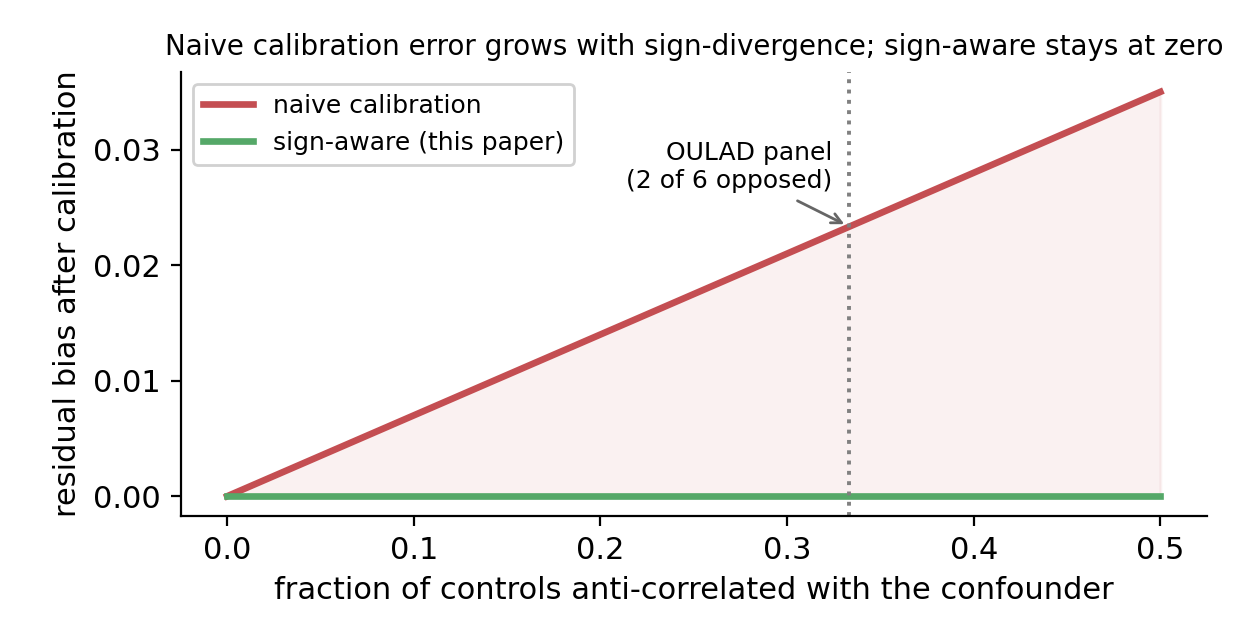
\includegraphics[width=.90\textwidth,height=.50\textheight,keepaspectratio]{../manuscript_updated/figures/figure_08.png}
\end{center}

The figure marks the fraction of flipped signs in the archived OULAD panel for reference. The observed control contrasts are heterogeneous, so that fraction alone cannot determine the sign or magnitude of the empirical correction. More generally, the contribution of an oppositely oriented control to the difference between the two population pools is twice its oriented bias divided by the panel size. One large control can therefore matter more than several weak controls.

\subsection{Archived known-truth benchmarks}

The original linear benchmark used 1,000 repetitions per setting, 4,000 learners per repetition, six controls and approximately equal bias magnitudes. The table gives the reported residual bias and coverage under ordinary and signed pooling. These results apply to the matched-magnitude benchmark and complement the magnitude and sign perturbations in the main text.

\subsection{What the evidence supports}

Sign alignment can prevent cancellation in a deliberately specified common-bias model. The simulation in Table~\ref{tab:simulation-results} supports conditional usefulness of the unchanged orientation/pooling rule. Its failures under different control magnitudes and incompatible factors show why the condition is consequential. A control's known zero causal effect does not imply that subtracting its association improves the target estimator.

\begin{table}[htbp]\centering\small
\caption{Known-truth binary simulation of the unchanged sign-aware/MoM rule. Each row uses 500 repetitions, $n=2000$ and two-fold AIPW with logistic working models. The non-null ATE is computed by quadrature.}\label{tab:simulation-results}
\begin{tabularx}{\textwidth}{Xrrrrr}\toprule Scenario & True ATE & Raw RMSE & Signed RMSE & Coverage & Reject 0 \\\midrule
Matched controls & 0.000 & 0.123 & 0.028 & 0.952 & 0.048 \\
Matched controls & 0.105 & 0.124 & 0.027 & 0.954 & 0.960 \\
Different magnitudes & 0.000 & 0.123 & 0.082 & 0.228 & 0.772 \\
Different magnitudes & 0.105 & 0.124 & 0.081 & 0.230 & 0.184 \\
Incompatible factors & 0.000 & 0.147 & 0.347 & 0.000 & 1.000 \\
Incompatible factors & 0.111 & 0.146 & 0.345 & 0.000 & 1.000 \\
No confounding & 0.000 & 0.024 & 0.025 & 0.948 & 0.052 \\
No confounding & 0.105 & 0.023 & 0.024 & 0.960 & 0.988 \\
\bottomrule\end{tabularx}\end{table}
At coverage 0.95, Monte Carlo standard error is about 0.010 for 500 repetitions. Rejection at true zero measures type-I error; at nonzero effects it measures power. 
\begin{figure}[htbp]\centering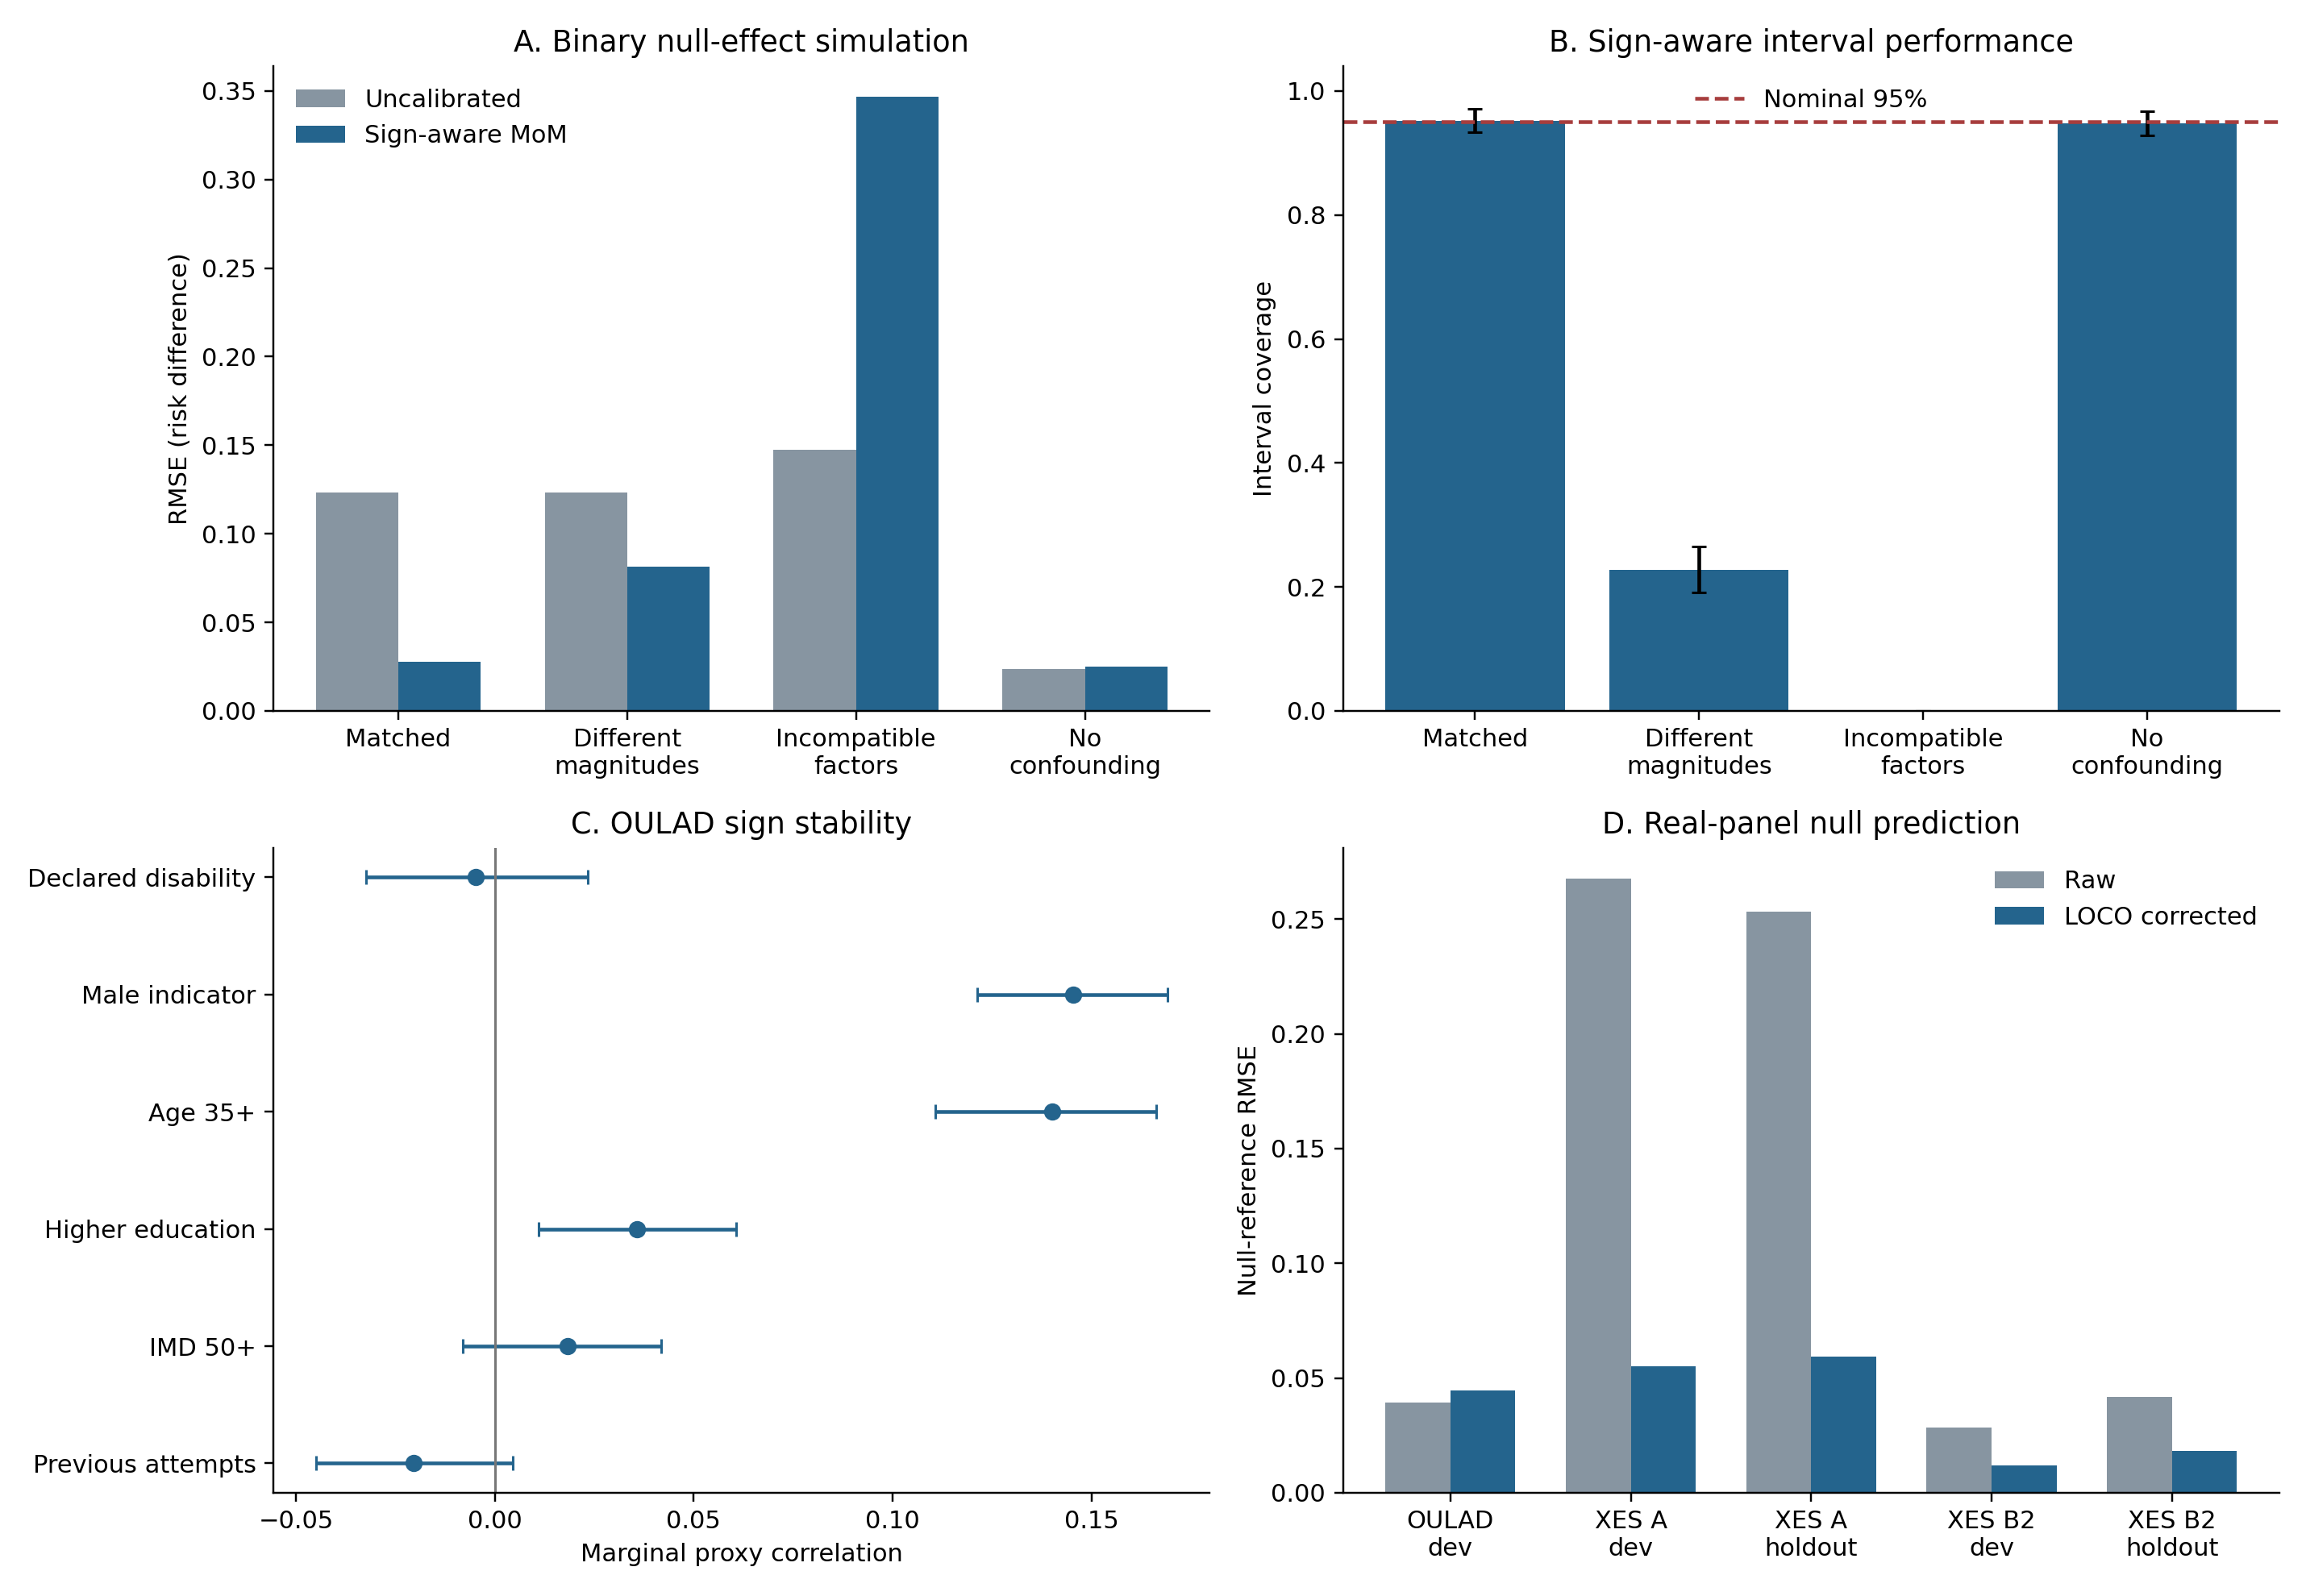
\includegraphics[width=\textwidth]{audit_summary.png}
\caption{Conditional simulation performance and real-panel diagnostics. Top: binary known-truth RMSE and nominal coverage (coverage bars show $\pm1.96$ Monte Carlo SE). Bottom left: OULAD cluster-bootstrap marginal correlations on full training keys. Bottom right: null-reference error before and after leave-one-control-out correction. Real-panel checks do not identify target bias.}\label{fig:audit-summary}\end{figure}

\subsection{Stress test of magnitude and orientation}
We extended the known-truth evaluation with a Gaussian experiment at the estimate level. The true effect is zero and the target estimator has population bias $0.06$ and standard error $0.025$. Six independent control estimates have standard errors $0.020$, alternating true orientations, and population magnitudes $0.06\lambda_k$. Sampling errors are mutually independent in this experiment. We evaluated $\lambda_k=1$, unequal loadings averaging one $(.25,.50,.75,1.25,1.50,1.75)$, weak controls $(.20,.30,.40,.50,.60,.70)$, and a single dominant control $(6,1,1,1,1,1)$. A separate perturbation reverses each orientation independently with probability $0.25$, with and without the dominant control. We used 30,000 draws per scenario and compared the uncorrected Wald interval with the same nominal MoM pooling interval for each correction.

\begin{table}[htbp]\centering\small
\caption{Gaussian stress test at a true effect of zero. Each method column gives bias, 95\% coverage, and false-positive rate, respectively.}\label{tab:gaussian-stress}
\begin{tabularx}{\textwidth}{Xlll}\toprule
Scenario & Raw & Unaligned & Aligned\\\midrule
Matched & +0.060, 33.2\%, 66.8\% & +0.060, 99.3\%, 0.7\% & +0.000, 94.8\%, 5.2\% \\
Unequal, mean one & +0.060, 33.2\%, 66.8\% & +0.070, 99.6\%, 0.4\% & -0.000, 99.5\%, 0.5\% \\
Weak controls & +0.060, 32.7\%, 67.3\% & +0.063, 68.1\%, 31.9\% & +0.033, 79.0\%, 21.0\% \\
Sign error & +0.060, 32.9\%, 67.1\% & +0.060, 99.3\%, 0.7\% & +0.030, 98.5\%, 1.5\% \\
Dominant control & +0.060, 33.6\%, 66.4\% & +0.010, 100.0\%, 0.0\% & -0.050, 100.0\%, 0.0\% \\
Dominant + sign error & +0.060, 33.0\%, 67.0\% & +0.010, 100.0\%, 0.0\% & +0.005, 100.0\%, 0.0\% \\
\bottomrule\end{tabularx}\end{table}

Unequal magnitudes can preserve the mean correction when they average to the target bias. Weak controls leave residual bias despite correct orientation. A dominant control can overcorrect the point estimate while inflating the pooled interval, so coverage alone can conceal poor correction. At a true zero effect, empirical coverage and false-positive rejection are complementary. This experiment isolates the pooling step under fixed target and control standard errors. The binary simulations above additionally exercise outcome modelling and cross-fitting.


The real-data analyses instead provide design diagnostics. They investigate fixed adjustment, shared support, explicit coding, known-null prediction and outcome definitions. Positive or negative observational contrasts are not known causal effects, and a change in nominal significance cannot establish calibration accuracy. Removing or retaining controls on the basis of a desired target result would not validate the method.

In the binary AIPW extension (Section~\ref{sec:binary-stress}), weak controls left signed bias of $+.075$ and a 66.2\% false-positive rate under the null. A dominant control yielded bias of $-.024$ with 99.6\% coverage and 2.34 times the uncorrected interval width. With a true effect of .105, the signed interval rejected zero in 96.0\% of matched-panel runs and 9.2\% of dominant-panel runs.

\subsection{Binary-outcome AIPW stress test}
\label{sec:binary-stress}

Each cell uses 500 independent samples of 2,000 learners. With independent standard normal variables $U,X,\epsilon,\eta$, treatment is $A=\mathbb{1}\{U+.5X+\epsilon>0\}$ and the measured orientation proxy is $G=U+\eta$. The target outcome has logit $\alpha A+.8U+.4X$. Control $j$ has logit $s_j(l_j U+.4X)$, with alternating $s_j=\pm1$ and no treatment term. The matched loadings are all .8. The weak loadings are $(.15,.20,.25,.30,.35,.40)$ and the dominant panel is $(3.2,.8,.8,.8,.8,.8)$. These are logit coefficients. Residual risk-difference biases also depend on adjustment and the nonlinear link.

The analysis fits logistic propensity and treatment-specific outcome models using $X,G$ in two cross-fitting folds, separately in each replication, and clips estimated propensities to $[.02,.98]$. The true marginal effect is computed by Gaussian quadrature for $\alpha=0$ and $\alpha=.5$. Signs are estimated from the target and control correlations with $G$ in each sample. The signed covariance interval for fixed estimated orientations is available in the replication files.

\begin{center}\small
\begin{tabular}{llrrrrr}\toprule
Panel & Method & ATE & Bias & Coverage & Reject zero & Width \\\midrule
Matched & Uncorrected & 0.000 & +0.121 & 0.006 & 0.994 & 0.104 \\
Matched & Ordinary & 0.000 & +0.120 & 1.000 & 0.000 & 0.528 \\
Matched & Signed & 0.000 & -0.001 & 0.952 & 0.048 & 0.114 \\
Matched & Uncorrected & 0.105 & +0.122 & 0.000 & 1.000 & 0.103 \\
Matched & Ordinary & 0.105 & +0.122 & 1.000 & 0.140 & 0.528 \\
Matched & Signed & 0.105 & +0.001 & 0.954 & 0.960 & 0.114 \\
Weak & Uncorrected & 0.000 & +0.121 & 0.006 & 0.994 & 0.104 \\
Weak & Ordinary & 0.000 & +0.124 & 0.362 & 0.638 & 0.224 \\
Weak & Signed & 0.000 & +0.075 & 0.338 & 0.662 & 0.124 \\
Weak & Uncorrected & 0.105 & +0.122 & 0.000 & 1.000 & 0.103 \\
Weak & Ordinary & 0.105 & +0.126 & 0.360 & 1.000 & 0.224 \\
Weak & Signed & 0.105 & +0.076 & 0.318 & 1.000 & 0.124 \\
Dominant & Uncorrected & 0.000 & +0.121 & 0.006 & 0.994 & 0.104 \\
Dominant & Ordinary & 0.000 & +0.097 & 1.000 & 0.000 & 0.659 \\
Dominant & Signed & 0.000 & -0.024 & 0.996 & 0.004 & 0.243 \\
Dominant & Uncorrected & 0.105 & +0.122 & 0.000 & 1.000 & 0.103 \\
Dominant & Ordinary & 0.105 & +0.098 & 1.000 & 0.000 & 0.659 \\
Dominant & Signed & 0.105 & -0.023 & 1.000 & 0.092 & 0.242 \\
\bottomrule\end{tabular}
\end{center}

\subsection{Semi-synthetic OULAD benchmark}

The semi-synthetic benchmark used OULAD covariates and the recorded pre-deadline engagement signal. The simulation assigned treatment through a mechanism driven by engagement and generated an outcome with a known average effect of approximately .123. The fitted nuisance models omitted the engagement variable used for confounding. Six generated control outcomes shared the engagement loading in magnitude, with four entering the pool in the opposite direction.

The raw, ordinary and signed estimates were .231, .270 and .120. We extended this benchmark using standardized pre-deadline log-click engagement $U_1$ and a generated independent standard normal factor $U_2$. Each panel used 500 samples of 2,000 distinct OULAD learners, taking the first registration per learner in module and presentation order. Measured covariates were module, presentation length and registration timing. With $B=.25$ times standardized length minus $.20$ times standardized registration timing, the treatment logit was $.9U_1+.8U_2+B$ and the target logit was $-.3+.85U_1+.65U_2+B+\alpha A$. Truth is the within-sample mean difference in potential outcome probabilities for $\alpha=0,.55$.

Six controls have logits $s_j(\ell_j^\top U+B)$, with two positive and four negative signs. Matched loadings are $(.85,.65)$; proportional multipliers are $(.25,.5,.75,1.25,1.5,1.75)$. Mixed loadings are $(.2,.1),(.4,-.4),(.6,.05),(1,-.8),(1.25,.15),(1.5,-1)$. Two-fold logistic AIPW refits all models in each sample using measured covariates and a noisy proxy $U_1+\epsilon$, with $\epsilon$ standard normal. The same proxy determines relative signs. Neither confounder enters the nuisance models directly.

\begin{center}\footnotesize
\begin{tabular}{llrrrrr}\toprule
Panel & Method & ATE & Bias & Coverage & Width & Reject zero \\\midrule
Matched & Raw & 0.000 & +0.143 & 0.000 & 0.091 & 1.000 \\
 & Ordinary & 0.000 & +0.192 & 1.000 & 0.595 & 0.000 \\
 & Signed & 0.000 & -0.002 & 0.964 & 0.099 & 0.036 \\
Matched & Raw & 0.109 & +0.146 & 0.000 & 0.091 & 1.000 \\
 & Ordinary & 0.109 & +0.194 & 1.000 & 0.595 & 0.562 \\
 & Signed & 0.109 & +0.000 & 0.956 & 0.098 & 0.992 \\
Proportional & Raw & 0.000 & +0.143 & 0.000 & 0.091 & 1.000 \\
 & Ordinary & 0.000 & +0.235 & 0.656 & 0.492 & 0.344 \\
 & Signed & 0.000 & +0.010 & 1.000 & 0.260 & 0.000 \\
Proportional & Raw & 0.109 & +0.146 & 0.000 & 0.091 & 1.000 \\
 & Ordinary & 0.109 & +0.238 & 0.602 & 0.492 & 0.998 \\
 & Signed & 0.109 & +0.012 & 1.000 & 0.260 & 0.378 \\
Mixed & Raw & 0.000 & +0.143 & 0.000 & 0.091 & 1.000 \\
 & Ordinary & 0.000 & +0.158 & 0.098 & 0.233 & 0.902 \\
 & Signed & 0.000 & +0.129 & 0.296 & 0.232 & 0.704 \\
Mixed & Raw & 0.109 & +0.146 & 0.000 & 0.091 & 1.000 \\
 & Ordinary & 0.109 & +0.160 & 0.086 & 0.233 & 1.000 \\
 & Signed & 0.109 & +0.131 & 0.314 & 0.232 & 1.000 \\
\bottomrule\end{tabular}
\end{center}
Rejecting zero measures false positives at ATE zero and power otherwise. This benchmark tests the chosen confounding structures on OULAD covariates. Empirical control comparability still requires a substantive argument.


At the null, signed pooling left bias of $-.002$ with matched loadings and $+.010$ with proportional loadings. Coverage rose from 96.4\% to 100\%, while mean interval width rose from .099 to .260. At a true effect near .109, rejection fell from 99.2\% to 37.8\%. With mixed loadings, signed bias reached $+.129$ at the null and 70.4\% of intervals excluded zero. The first-factor proxy can orient the controls along that factor while the second factor contributes bias in a different direction.


\section{Discussion}
\subsection{What remains unverified}

There is no demonstrated equality between the target's residual bias and the mean oriented control bias in either dataset. Proxy correlations are not direct measurements of that quantity; multiple confounders, different pathways, nonlinear links and measurement error can break the connection. The no-treatment-effect condition for baseline attributes is stronger than the corresponding timing argument for sequence-derived XES summaries, whose observation process needs additional care.

Small panels cannot support a reliable normal empirical-null interpretation without further evidence. Estimated signs and empirical-null parameters add uncertainty, while controls are measured on the same people. A shared-score covariance calculation addresses dependence under fixed estimated signs, but does not solve identification. The MoM nominal intervals have no new theorem of causal coverage in this study. The binary simulation uses particular working models and does not establish universal performance for arbitrary retention mechanisms.

In OULAD, a feature observed before the deadline may nevertheless follow the actual submission of an early submitter. Thus a deadline-restricted click window is not automatically a pre-exposure window for every individual. Establishing a well-defined treatment time and appropriate baseline covariates is a further requirement for an intervention interpretation; the present common-design analysis is a diagnostic observational audit.

The archived real-data estimates are not substituted for the new audit. Input provenance, endpoint definitions, temporal cutoffs and weighting need to match before a numerical result can be treated as reproduced. These reproducibility conditions are necessary before making a substantive case for control comparability.

\subsection{What interval width reveals}

The semi-synthetic experiment separates two sources of difficulty. Heterogeneous proportional loadings change the magnitude of the bias contributed by each control while preserving the direction of its loading vector. The multipliers average one on the logit scale. The resulting risk-difference biases depend on the nonlinear outcome link, the exposure mechanism and the AIPW adjustment, so their average can still differ from the target bias. With mixed loadings, the second factor can push a control contrast in a direction that the proxy for the first factor cannot capture. Even a reproducible proxy sign gives limited information about the direction of the total residual bias.

The method-of-moments interval adds the estimated spread of the oriented control contrasts to the target variance. A second calculation uses the covariance of the target and control influence scores, conditional on the estimated signs. The latter quantifies sampling variation for the signed contrast with orientations treated as fixed. It addresses shared observations across outcomes. It omits uncertainty from sign estimation and from the difference between the target bias and the mean oriented control bias. Both calculations use the same point estimate within each replication.

\begin{table}[htbp]
\centering\small
\caption{Intervals for signed pooling in the OULAD semi-synthetic experiment at a true effect of zero. Width is in risk-difference units. Coverage and rejection are proportions over 500 replications per panel.}
\begin{tabular}{llrrr}
\toprule
Panel & Interval & Width & Coverage & Reject zero\\
\midrule
Matched & Method of moments & .099 & .964 & .036\\
Matched & Score covariance & .093 & .952 & .048\\
Proportional & Method of moments & .260 & 1.000 & .000\\
Proportional & Score covariance & .093 & .932 & .068\\
Mixed & Method of moments & .232 & .296 & .704\\
Mixed & Score covariance & .099 & .000 & 1.000\\
\bottomrule
\end{tabular}
\end{table}

With proportional loadings, the method-of-moments interval is nearly 2.8 times as wide as the covariance interval. Its high coverage accompanies the low rejection rate at a nonzero effect observed in the previous section. In the mixed panel, the covariance interval is centered on a contrast with residual bias of about .129 and has mean width .099. All 500 covariance intervals exclude zero. Allowing the control spread to widen the interval reduces rejection to 70.4\%, still far above the nominal 5\%. The comparison isolates a difference in interval construction because the estimated correction and signs are identical for the two intervals within each replication. For the mixed-panel method-of-moments result, the Monte Carlo standard error of the rejection rate is approximately two percentage points.

\subsection{Position of the contribution}

The orientation step is a simple methodological modification. The applied contribution is to expose its assumptions and examine them in educational-data designs, including unfavourable checks. It is not claimed to supersede COCA, confounding-bridge estimation or general empirical calibration. Those methods make different identifying and error-model assumptions; a broader comparison requires their actual implementations and matching estimands.

Further evidence would include a substantively justified homogeneous control family, independent information about how its confounding relates to the target, or a benchmark with a credible causal reference effect. Repeated simulations that impose equality of bias magnitudes cannot supply that external evidence. If a panel fails the rationale or diagnostics, its members remain useful for bias detection but their pooled mean should not be represented as validated target-bias correction.

\section{Conclusion}

Orientation before negative-control pooling has conditional value, but cannot establish that heterogeneous outcomes measure commensurable residual bias. An exact MSE decomposition separates bias reduction from precision improvement. Known-truth simulations show both success and failure of the retained rule. Common-design real-data audits improve transparency about inputs, controls and estimator comparability while leaving causal identification unresolved. The appropriate claim is conditional calibration and diagnostic assessment, with explicit limitations on what the educational-data results establish.

\section*{Data and code availability}

The revision includes the audit analysis plan, raw-source checksums, code fingerprints, aggregate control results and known-truth simulation outputs. OULAD and XES3G5M are described by their original dataset publications. Student identifiers and raw records are not reproduced in the manuscript. The new real-data audit is post-screening work; it is not described as an externally preregistered analysis. Archived source gaps and unverified input provenance are recorded in the accompanying revision memo rather than silently claimed as complete reproduction.

\section*{Conflicts of interest}
The authors declare no competing interests.
